In this chapter we introduce a representation of static and dynamic graphs suitable to characterize graphs in the \dpm. 
A particular property of \msts\ represented as we propose will allow us to compute the \mst\ of a graph in the \dpm. 
We show also the \DPmst\ Algorithm that uses this representation for tailor the \dpm, and delve into its detailed 
implementation and various optimizations. 
We begin by explaining the representation and proving the above mentioned property, 
followed by its usage in the dynamic pipeline with a comprehensive breakdown of the implementation, 
which includes the Communication, Source Stage, Filter Stage, Generator Stage, and Sink Stage.
Afterwards we include a cost analysis section, where we evaluate the time and memory complexity of \DPmst, 
providing insights into its efficiency and scalability.
We then introduce several key optimizations designed to enhance the performance of \DPmst. 
These include the use of multiple roots per filter, Decoupled Event Handling, adaptive \mst\ caching, and improved memory management. Notably, the Decoupled Event Handling optimization is highlighted as a general improvement that can be applied to any problem implemented using the \dpm, not just the \mst\ problem.

Through these sections, we aim to demonstrate how the \DPmst\ algorithm, bolstered by these optimizations, offers a robust and scalable solution for maintaining the \mst\ in dynamic graphs. This sets the stage for the experimental analyses presented in subsequent chapters, where the effectiveness of these enhancements is empirically validated.

\section{Underlying Forests and \msts}
In this section we present our algorithm for computing minimum spanning forests of dynamic 
weighted graphs according to the dynamic pipeline approach. 
In order to simplify the following definitions, we assume that the graphs have no isolated vertices (vertices with no incident edges), 
but can be easily adapted. We start by introducing the preliminaries to define the algorithm. 

In the literature~\cite{Cormen4thEdition}, there are many possible computational representations of graphs: 
as adjacency lists, as adjacency matrices, as a computable function, as a list of edges and many more. 
We propose a representation based on its \emph{underlying forest}.

\begin{definition}\label{def:u-forest}
Given a graph $G=(V,E)$, we say that the sequence $F_G = \langle T_1,\dots,T_k\rangle$, $k \ge 1$, 
is an \emph{underlying forest} of $G$ 
if $T_i \subseteq E$ $\forall i$, $\cup_{i=1}^k T_i = E$, $\forall i,j, i\neq j, T_i\cap T_j = \emptyset$
and  $\forall i\:\: T_i\in F_G$ there exists a distinguished vertex $v_i\in V$, called the \emph{root} 
of $T_i$, such that $\forall e \in T_i$,  $e$ is incident to $v_i$.
\end{definition}
 
Notice that every element of an underlying forest of $G$ is a tree of height 1. Indeed, 
$\forall T_i \in F_G\:\: \mathsf{height}(T_i)=1$. Notice also that if $T_i$ consists of a unique edge 
any of its two vertices could be distinguished as the root of $T_i$.
Moreover, $G$ can be characterized as $G=(V,\bigcup_{j=1}^k T_j), k\ge 1$ and hence, 
in what follows, by an abuse of notation we might also write  $G = \bigcup_{i=1}^k T_i$. 
Likewise, we will also refer by $G_i$ to the graph of $G$ given by $G_i = \bigcup_{j=1}^i T_j$, $1\leq i\leq k$.

%%%%%%%OLD
%\begin{definition}\label{def:u-forest}
%Given a graph $G=(V,E)$, an \emph{underlying forest} of $G$,  $F_G = \langle T_1,\dots,T_k\rangle, k \ge 1$ is the sequence induced by a %partition of the set of edges $E$, where $\forall i\:\: T_i\in F_G$ there exists a distinguished vertex $v_i\in V$, called the \emph{root} %of $T_i$ such that $\forall e \in T_i$,  $e$ is incident to $v_i$ .
%\end{definition}
 
%Notice that, since in an underlying forest $\forall T_i \in F_G\:\: \mathsf{height}(T_i)=1$ and if $T_i$ has only one edge both of their incidents vertices can be distinguished as the root of $T_i$.
%Moreover, because of $F_G$ is a partition of $E$, we can characterize $G$ as $G=(V,\bigcup_{j=1}^k T_j), k\ge 1$ and hence, in what follows, by an abuse of notation we we will also write  $G = \bigcup_{i=1}^k T_i$. Also, similar to this abuse of notation, we will also refer as the subgraph $G_i$ of $G$ to the graph produced by $G_i = \bigcup_{j=1}^i T_j $.


In Figure~\ref{fig:graph-and-mst}, we show a weighted graph $G$ together with one of its possible underlying forests. 
Edges are represented by 3-tuples of the form $(u,v,\omega(\{u,v\}))$, where $\omega(\{u,v\})$ is the cost of the edge $\{u,v\}$ (according to Definition~\ref{def:wgraph}). The graph therein is 
$G=(V,E)$, with $V= \{a,b,c,d,e\}$ and 
$E= \{(a,b,2),$ $(a,e,1),(b,e,1),$ $(c,e,1),(b,d,7),(c,d,4),(b,c,1)\}$. 

\begin{figure}[H]
\begin{center}
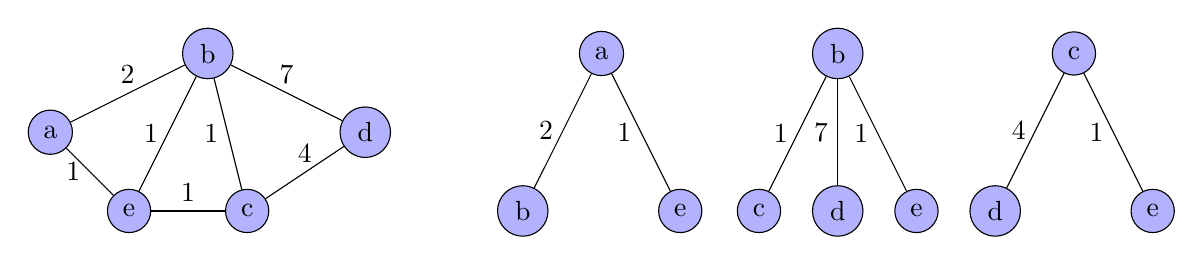
\begin{tikzpicture}
    \node[shape=circle,draw=black, fill = blue!30] (a) at (-3,0) {a};
    \node[shape=circle,draw=black, fill = blue!30] (b) at (-1,1) {b};
    \node[shape=circle,draw=black, fill = blue!30] (c) at (-0.5,-1) {c};
    \node[shape=circle,draw=black, fill = blue!30] (d) at (1,0) {d};
    \node[shape=circle,draw=black, fill = blue!30] (e) at (-2,-1) {e};

    \path [-] (a) edge node[above] {$2$} (b);
    \path [-](a) edge node[left] {$1$} (e);
    \path [-](b) edge node[left] {$1$} (e);
    \path [-](b) edge node[left] {$1$} (c);
    \path [-](b) edge node[above] {$7$} (d);
    \path [-](c) edge node[above] {$4$} (d);
    \path [-](e) edge node[above] {$1$} (c);  

    \node[shape=circle,draw=black, fill = blue!30] (f) at (4,1) {a};
    \node[shape=circle,draw=black, fill = blue!30] (g) at (3,-1) {b};
    \node[shape=circle,draw=black, fill = blue!30] (h) at (5,-1) {e};
  
    \path [-] (f) edge node[left] {$2$} (g);
    \path [-](f) edge node[left] {$1$} (h);

    \node[shape=circle,draw=black, fill = blue!30] (i) at (7,1) {b};
    \node[shape=circle,draw=black, fill = blue!30] (j) at (6,-1) {c};
    \node[shape=circle,draw=black, fill = blue!30] (k) at (7,-1) {d};
    \node[shape=circle,draw=black, fill = blue!30] (l) at (8,-1) {e};
  
    \path [-] (i) edge node[left] {$1$} (j);
    \path [-](i) edge node[left] {$7$} (k);
    \path [-](i) edge node[left] {$1$} (l);

    \node[shape=circle,draw=black, fill = blue!30] (m) at (10,1) {c};
    \node[shape=circle,draw=black, fill = blue!30] (n) at (9,-1) {d};
    \node[shape=circle,draw=black, fill = blue!30] (o) at (11,-1) {e};
  
    \path [-] (m) edge node[left] {$4$} (n);
    \path [-](m) edge node[left] {$1$} (o);
\end{tikzpicture}
\caption{\label{fig:graph-and-mst}The sequence of trees on the right form an underlying forest of the graph shown in the left.}
\end{center}
\end{figure}

This characterization allows to analyze various properties of graphs in the \dpm, however, our interest is to study the way to compute and maintain dynamically the \mst\ of a dynamic graph. To do so, next proposition is crucial.

%From this definition, we can analyze various properties of graphs with this representation. Specifically, next proposition give us the %basis for developing and algorithm for, given a weighted graph $G$,  computing \mstof{G} supported on Definition \ref{def:u-forest}.

\begin{proposition} 
\label{prop:recursive_mst}
Given a weighted graph $G=(V,E)$ represented by the underlying forest 
$F_G = \langle T_1, \dots, T_k\rangle\ (k \ge 1)$ and the subgraphs $G_i$, $1\leq i\leq k$, of $G$ 
such that $G_i = \cup_{j=1}^kT_i$, it holds that
    \[
        \mathsf{MST}(G_i) =     \left\{ \begin{array}{lr}
				                    T_1& \mbox{if}\:\: i = 1 \\ 
				                    \mathsf{MST}(T_i \cup \mathsf{MST}(G_{i-1})) & \mbox{if}\:\: i > 1 \\
			                \end{array}\right.
    \]
where \mst(G) is any correct procedure to compute a \mst\ of $G$.
\end{proposition}

\begin{proof}
    We proceed by induction on the size of  $F_G$.

    \emph{Base case, i= 1}: $F_{G_1} = \langle T_1\rangle$ and thus $G_1 = T_1$. Since $T_1$ is a tree containing all the edges of $G_1$, 
    it corresponds to its own minimum spanning tree.
    Let us observe that for the case $i=2$ the property follows trivially since $\mathsf{MST}(G_2) = \mathsf{MST}(T_1\cup T_2) = \mathsf{MST}(\mathsf{MST}(T_1)\cup T_2)$.

    \emph{Induction Hypothesis (HI)}: Let us suppose that $\mathsf{MST}(G_{i})=\mathsf{MST}(T_{i} \cup \mathsf{MST}(G_{i-1}))$ is,  
    effectively, a \mst\ of $G_i$.

    We want to proof that if (HI) holds then $\mathsf{MST}(G_{i+1})=\mathsf{MST}(T_{i+1} \cup \mathsf{MST}(G_{i}))$.
    
    \emph{Induction Step}:
    Let $e\in E$ be any edge of $\mathsf{MST}(G_{i+1})$, then $e$ is either in $G_i$ or in $T_{i+1}$ 
    If $e$ belongs to $T_{i+1}$, then $\mathsf{MST}(G_{i+1})$ will consider it (since it looks at all the edges of $T_i$) and add it to $\mathsf{MST}(G_{i+1})$.

    If, on the other hand, $e$ belongs to $G_i$ then there are two options for it to belong to $\mathsf{MST}(G_{i+1})$:
    \begin{enumerate}[1)]
        \item $e$ does not belong to any cycle in $G_{i+1}$, which implies that the edge does not belong neither to any cycle in $G_i$, 
        so it will also be part of $\mathsf{MST}(G_i)$ and hence will be considered by $\mathsf{MST}(G_{i+1})$.
        \item $e$ belongs to at least one cycle of $G_{i+1}$. If $e$ belongs only to cycles that include  
        edges from $T_{i+1}$, then as $G_i$ does not include such edges, $e$ does not belong to any cycle in $G_i$ and hence has to be part of $\mathsf{MST}(G_i)$. 
        The last option left is that the $e$ belongs to cycles in $G_i$. In such case, it cannot be the weightiest edge in any of that cycles, otherwise it would not be part of $\mathsf{MST}(G_{i+1})$, hence it has to be in $\mathsf{MST}(G_i)$.
    \end{enumerate}
    With all this cases covered, we can state that we can build the $\mathsf{MST}(G_{i+1})$ as the \mst\ of the union of the tree $T_{i+1}$ with the $\mathsf{MST}(G_i)$.

    We have not considered here the case in which the graphs $G_i$, $1\leq i\leq k$, are not connected. 
    If this is the case, then the final result is the sequence of \msts\ of every connected component of $G_i$. 
    Since the proposition holds for any connected component, it is valid for the union of all connected components. 
\end{proof}

Proposition~\ref{prop:recursive_mst} gives us the foundation to compute the \mst\ of graphs 
represented by any of their underlying forests. To get insights about how this can help us to design an algorithmic proposal,  
let us consider the Example~\ref{example:mst1}.

\begin{example} [Computation of $\mathsf{MST}(G)$ from $F_G$]
\label{example:mst1}
Let $G$ be the forest $F_G=\langle T_1, T_2, T_3\rangle$, where $T_1= \{(a,b,2),(a,e,1)\}$, $T_2= \{(b,c,1),(b,d,7),(b,e,1)\}$ and, $T_3 = \{(c,d,4) ,(c,e,1)\}$ shown in Figure~\ref{fig:graph-and-mst}. The computation of $\mathsf{MST}(G)$ is done according to Proposition \ref{prop:recursive_mst}. This is, $\mathsf{MST}(G)$ is $\mathsf{MST}(T_3)$ and is computed as follows:  
\begin{enumerate}
\item $\mathsf{MST}(G_1) = T_1 = \{(a,b,2),(a,e,1)\}$
\item $\mathsf{MST}(G_2) = \mathsf{MST}( T_2 \cup \mathsf{MST}(G_1) ) = \{(a,e,1), (b,c,1), (b,d,7), (b,e,1)\}$
\item $\mathsf{MST}(G_3) = \mathsf{MST}( T_3 \cup \mathsf{MST}(G_2) ) = \{(a,e,1), (b,c,1), (b,e,1), (c,d,4)\}$ 
\end{enumerate}
\end{example}

% DPA and  MSTs of Dynamic Graphs
\section{\dpm\ and \msts\ of Dynamic Graphs.} 
In the classical sequential model of computation one could easily implement the traversal of forest $F_G$ by a simple loop running over its trees. However, thinking in alternative ways of computation, it would be natural to distribute the trees of $F_G$ along a pipeline, distributing the sequence among several processors. Then, the sequence of computations given in Example~\ref{example:mst1} would also been distributed along the processors holding the trees implied in the computation. That is exactly the idea of the \emph{dynamic pipeline}, \DPmst. The benefit of using this graph representation is threefold: 
\begin{enumerate}[(i)]
    \item The graph can be updated in a very simple way, just by adding or deleting edges of one element of $F_G$. Moreover, as we will see, this representation is adequate for the \dpm~\cite{Pasarella2024} since the trees of $F_G$ can be very easily spread out across a {\em dynamic pipeline} producing the distributed representation of the graph that we will refer to as \DPmst. Hence, while the dynamic pipeline is active, $G$ remains updated along time.

    \item  At any  time $t$, the concurrent (and parallel) computational structure of \DPmst\ is able to compute effectively the $\mathsf{MST}(G)$ of the current graph when required.

    \item During the computation of the $\mathsf{MST}(G)$, the priority queue required for the implementation is of size at most $O(n)$ in contrast with the sized $m$ priority queue required by the implementation of Kruskal's sequential algorithm because there will be at most $2n$ edges.
\end{enumerate}

Following the definition in~\cite{Pasarella2024}, to define a dynamic pipeline, we have to define (i) the configuration and the behaviour of the four kind of  different stages (\emph{stateful functions}): source or input, generator,  (instances of) filter and sink or output, in this order; and (ii) the channels connecting stages. Each filter instance's state contains a tree of the forest $F_G$ and is parameterized by the root of this tree. Besides filter instances' behaviour  correspond to the operation defined in Proposition~\ref{prop:recursive_mst}. The different stages of the pipeline are connected by means of two communication channels carrying the {\em events} and the  $\mathsf{MST}(T_k)$ for passing the temporal $\mathsf{MST}(G)$, respectively.

When a pipeline is initialised, only the Source, the Generator and the Sink stages exist. Then, the pipeline shrinks and expands dynamically depending on the sequence of insertions and deletions of the edges of the graph but all these operations can modify only the number of filter stages, the underlying structure is not modified, unless the \DPmst\ terminates. Figure \ref{fig:dp_example} depicts the state of an instance of \DPmst, and below we describe all the stages with more precision.

\emph{Source ($I$)}: Whenever this stage receives an event it passes 
        it to the rest of the pipeline through the event channel, if ${\tt op} =\opmst$
        it also passes the empty set through the graph channel.

\emph{Filter ($F(v)$)}: The parameter $v$ is called the \emph{root} of the 
        filter stage. Whenever an event $({\tt op,e=\{v,w\})}$ arrives to $F(v)$, the following things
        can happen:  (i) If ${\tt op}=\{{\tt insert, update, delete}\}$ and $e$ is incident to
        the root $v$, the event is treated in $F(v)$ according to ${\tt op}$. On the contrary, if it is not incident, the event is passed through the event channel to the next
        stage of the pipeline; (ii) If ${\tt op}=\opmst$,  a partial \mst\ is computed and
        passed to the rest of the pipeline through the graph channel by 
        computing the \mst\ of the graph resulting of the union of the 
        \mst\ that arrives through the graph channel with the tree in $F(v)$. As explained, a possible implementation would consist on joining the temporal graph from the graph channel with the filter's tree and the compute the \mst\ with Kruskal's algorithm.
        
\emph{Generator ($Gen$)}: Whenever an event $({\tt op,e=\{v,w\}})$ arrives to this stage  
        by the event channel, if ${\tt op}\in\{{\tt insert, update}\}$, a new instance of
        Filter stage, $F(v)$, is spawned and added to the pipeline 
        between the last filter and $Gen$. The edge $e$ is stored in the local memory of $F(v)$. Besides, whenever 
        ${\tt op}=\opmst$, it passes the \mst\ that arrives by the graph channel 
        to the sink stage $O$.
        
\emph{Sink ($O$)}: When an event $\opmst$ arrives to this stage, it outputs the \mstof{G}.

\begin{figure}[H]
    \centering
    %Input Graph
    \begin{subfigure}[b]{0.20\textwidth}
    \centering
    \resizebox{\textwidth}{!}{
    \begin{tikzpicture}
        \begin{pgfonlayer}{nodelayer}
            \node[style=new style 0] (a) at (0,0) {a};
            \node[style=new style 0, left=1cm of a] (b) {b};
            \node[style=new style 0, above right=1.118cm of a] (c) {c};
            \node[style=new style 0, below right=1.118cm of a] (d) {d};
            \node[style=new style 0, right=1cm of c] (e) {e};
            \node[style=new style 0, right=1cm of d] (f) {f};
        \end{pgfonlayer}
        \begin{pgfonlayer}{edgelayer}
            \draw[style={tree_edge}]{} (b) to["0.4"] (a);
            \draw[style={tree_edge}]{} (c) to["0.3"] (d);
            \draw[style={tree_edge}]{} (a) to["0.6"] (c);
            \draw[style={tree_edge}]{} (d) to["0.1"] (f);
            \draw[style={tree_edge}]{} (d) to["0.8"] (a);
            \draw[style={tree_edge}]{} (c) to["0.9"] (e);
        \end{pgfonlayer}
    \end{tikzpicture}
    }    
    \end{subfigure}
    % DP
    \begin{subfigure}[b]{0.55\textwidth}
    \centering
    \resizebox{\textwidth}{!}{
    \begin{tikzpicture}
        \begin{pgfonlayer}{nodelayer}
            \node [style=io, minimum height=0.8cm, minimum width=3cm, shape border rotate=270] (In) at (0, 0) {I};
            \node [style=filter_gen, minimum width=1.5cm, minimum height=2.5cm, right= 0.6cm of In,  text depth = 1cm] (F1) {$F_a$};
            \node [style=filter_gen, minimum width=1.5cm, minimum height=2.5cm, right= 0.6cm of F1,  text depth = 1cm] (F2) {$F_c$};
            \node [style=filter_gen, minimum width=1.5cm, minimum height=2.5cm, right= 0.6cm of F2,  text depth = 1cm] (F3) {$F_d$};
            \node [style=filter_gen, minimum width=0.8cm, minimum height=2.5cm, align=center, right= 0.6cm of F3] (Gen) {Gen};
            \node [style=io, minimum height=0.8cm, minimum width=3.2cm, shape border rotate=90, right= 0.6cm of Gen] (Out) {O};
        \end{pgfonlayer}
        \begin{pgfonlayer}{edgelayer}
                \draw [style={opChan}] ([yshift=0.5 cm]Gen.east) to["Op"] ([yshift=0.5 cm]Out.west);
                \draw [style={daChan}] ([yshift=-0.5 cm]Gen.east) to["\mst\ "] ([yshift=-0.5 cm]Out.west);

                \draw [style={opChan}] ([yshift=0.5 cm]In.east) to["Op"] ([yshift=0.5 cm]F1.west);
                \draw [style={daChan}] ([yshift=-0.5 cm]In.east) to["\mst\ "] ([yshift=-0.5 cm]F1.west);
                
                \draw [style={opChan}] ([yshift=0.5 cm]F1.east) to["Op"] ([yshift=0.5 cm]F2.west);
                \draw [style={daChan}] ([yshift=-0.5 cm]F1.east) to["\mst\ "] ([yshift=-0.5 cm]F2.west);
                
                \draw [style={opChan}] ([yshift=0.5 cm]F2.east) to["Op"] ([yshift=0.5 cm]F3.west);
                \draw [style={daChan}] ([yshift=-0.5 cm]F2.east) to["\mst\ "] ([yshift=-0.5 cm]F3.west);
                \draw [style={opChan}] ([yshift=0.5 cm]F3.east) to["Op"] ([yshift=0.5 cm]Gen.west);
                \draw [style={daChan}] ([yshift=-0.5 cm]F3.east) to["\mst\ "] ([yshift=-0.5 cm]Gen.west);
        \end{pgfonlayer}

        \begin{pgfonlayer}{embeded}
            %Filter 1
            \node [style=new style 0, scale=0.5] (a1) at (1.75, -0.1) {a};
            \node [style=new style 0, scale=0.5,below=0.18cm of a1] (b1) {b};
            \node [style=new style 0, scale=0.5,below left=0.4cm of a1] (c1) {c};
            \node [style=new style 0, scale=0.5,below right=0.4cm of a1] (d1) {d};
            \draw[style={tree_edge}]{} (a1) to (b1);
            \draw[style={tree_edge}]{} (a1) to (c1);
            \draw[style={tree_edge}]{} (a1) to (d1);
            
            %Filter 2
            \node [style=new style 0, scale=0.5] (c2) at (3.9, -0.1) {c};
            \node [style=new style 0, scale=0.5,below left=0.4cm of c2] (d2) {d};
            \node [style=new style 0, scale=0.5,below right=0.4cm of c2] (e2) {e};
            \draw[style={tree_edge}]{} (c2) to (d2);
            \draw[style={tree_edge}]{} (c2) to (e2);
            
            %Filter 3
            \node [style=new style 0, scale=0.5] (d3) at (6.05, -0.1) {d};
            \node [style=new style 0, scale=0.5,below=0.18cm of d3] (f3) {f};
            \draw[style={tree_edge}]{} (d3) to (f3);
        \end{pgfonlayer}
    \end{tikzpicture}
    }
    \end{subfigure}
    %\hfill
    %Output MST
    \begin{subfigure}[b]{0.20\textwidth}
    \centering
    \resizebox{\textwidth}{!}{
    \begin{tikzpicture}
        \begin{pgfonlayer}{nodelayer}
            \node[style=new style 0] (a) at (0,0) {a};
            \node[style=new style 0, left=1cm of a] (b) {b};
            \node[style=new style 0, above right=1.118cm of a] (c) {c};
            \node[style=new style 0, below right=1.118cm of a] (d) {d};
            \node[style=new style 0, right=1cm of c] (e) {e};
            \node[style=new style 0, right=1cm of d] (f) {f};
        \end{pgfonlayer}
        \begin{pgfonlayer}{edgelayer}
            \draw[style={tree_edge}]{} (b) to["0.4"] (a);
            \draw[style={tree_edge}]{} (c) to["0.3"] (d);
            \draw[style={tree_edge}]{} (a) to["0.6"] (c);
            \draw[style={tree_edge}]{} (d) to["0.1"] (f);
            \draw[style={tree_edge}]{} (c) to["0.9"] (e);
        \end{pgfonlayer}
    \end{tikzpicture}
    }    
    \end{subfigure}
    \caption{\label{fig:dp_example} A \DPmst\ at some point of its execution, the input graph and the \mst\ that it returns. The graph is distributed along filters $F_a$, $F_c$ and $F_d$.} 
\end{figure}
%
\paragraph{Complexity.}
Conducting a precise cost analysis is inherently challenging due to the numerous influencing factors. In particular, the order in which graph modifications occur and the frequency of each type of operation significantly impact the structure of the pipeline and the overall performance. The following analyses provide a rough approximation based on the worst-case scenario and some amortised cost, ignoring the fact that we need to pass through all the filters. The \opinsert\  event is simply $O(1)$, since we are appending to the tree. The \opupdate\ and \opremove\ require to scan the list of adjacent edges of a tree, so it will be $O(n)$. The \opmst\ can be implemented using the Kruskal Algorithm of Section~\ref{sec:mst:kruskal}. Each tree has at most $n$ edges and the Kruskal Algorithm takes $O(n\log n)$ as mentioned in Section~\ref{sec:mst:kruskal}. This operation is performed at most $n$ times as there are at most $n$ trees in the underlying forest. So it has a cost $O(n^2 \log n)$, but the each operation in the trees can be performed in parallel for several \msts, which implies that we have an amortised cost of $O(n \log n)$. Each \opmst\ operation takes at most $O(n)$ memory since the resulting \mst\ has that size, the input graph as well and the priority queue needed for Kruskal takes also $O(n)$.
%
\section{Implementation}
The implementation was done using \Golang\ 1.20 and it is available at Github \footnote{\href{https://github.com/danielbenedi6/MasterThesis}{https://github.com/danielbenedi6/MasterThesis}}. The choice of \Go\ was influenced by several factors. Firstly, the language supports lightweight green threads called \texttt{goroutines}, which are efficiently managed by the \Go\ runtime scheduler. Additionally, the communication between stages is naturally facilitated by channels, enabling unidirectional communication between \texttt{goroutines}.

\subsection*{Communication}

To communicate between stages, as already explained, we use \Go\ channels. To avoid undesired synchronizations, we use buffered channels with up to 4096 item, a totally arbitrary number. Then, we packed the channels in \verb|in_comm| if the channels are only incoming and \verb|out_comm| for out-coming as shown in Figure \ref{code:channels}.

\begin{figure}[H]
    \centering
    \resizebox{0.4\textwidth}{!}{
    \lstinputlisting[language=Go]{code/channels.go}
    }
    \caption{Source code for the Channels in \Go.}
    \label{code:channels}
\end{figure}

\subsection*{Source Stage\label{sec:dp:input}}
The source stage consists of an element that will feed the pipeline either reading an input file or by generating random graphs, so-called in-memory.

When reading from a file, we defined a file format in order to unify the different formats from all the dynamic graph databases that we used. Although we started with a version that stated the operation with a keyword, we opted to change this definition because of performance issues. Instead, the operation is defined by an integer: the insert an edge operation is represented by number 1, the update the weight operation is number 2, the delete an edge operation is defined by number 3, the operation to obtain the minimum spanning tree is number 4, the number 5 represents the end of the file and the number 6 returns the whole graph. The operations of inserting and updating will be followed by three arguments representing the two vertices and the weight of the edge. The operation of deleting will be followed by the two vertices that form the edge.

\Golang\ offers different methods to parse data from a file. The most straightforward is based on the package \verb|fmt| in which we can simply define the format of the desired input and it will manage all the exceptions and ensure the parsing is correct. Another option is the package \verb|bufio| that allows to implement a parser and uses buffers to access to the files. An experimental analysis of both packages and why \verb|bufio| was chosen is given in~\ref{sec:exp:input}.

When the source stage is chosen to be a generator of random graphs, we opted to use binomial random graphs. A binomial random graph is a graph constructed by connecting nodes randomly in which each edge is included in the graph with probability $p$, independently from every other edge. A detailed explanation in Section \ref{sec:exp:rand_graph}.

Since both vertices of an edge can be the root in the underlying forest, before sending the edge through the \DPmst, a "normalization" operation is done in which the vertices are ordered lexicographically, so the smallest one will be the root. This order, instead of a random order for instance, affects the shape of the pipeline and it will be studied in Section~\ref{sec:edge_order}.

\subsection*{Filter Stage}

The filter stage is a functional stage, as defined in~\cite{Pasarella2024}, responsible for processing input data. The size of the \DPmst\ structure depends entirely on the number of filter stages present.

The grouping property, $\mathcal{R}$, of our filter stage ensures that each edge is adjacent to the root of the filter. Consequently, the filter retains only events with an adjacent edge. Instead of checking both vertices, we opted to check only the first vertex of the edge. The \opinsert\ operation adds the edge to the end of the edge list, $T_i$. The \opremove\ operation replaces the edge with the last one in the list and reduces the array size. The \opupdate\ operation scans the edge list and updates the edge weight.

The \opmst\ operation is more complex as it involves implementing an \mst\ algorithm and merging two trees. We assume the incoming \mst, $K$, is a sorted list of edges by weight. The operation then performs the Kruskal algorithm, as explained in Algorithm~\ref{alg:kruskal}. To find the connected component in which a vertex belongs to, we proposed the usage of the Union-Find data structure described in Algorithm~\ref{alg:unionfind}. Instead of selecting the lightest edge of the graph, the algorithm selects the lightest edge from either $K$ or $T_i$. Algorithm~\ref{alg:DPKRUSKAL} provides a pseudocode of a possible implementation of this process.

\begin{algorithm}
\caption{Possible implementation of Kruskal for Filter Stage of \DPmst\ \label{alg:DPKRUSKAL}}
\begin{algorithmic}
    \Require $T_i$ and $\mathsf{MST}(G_{i-1})$ are represented as a sequence of the edges and $\mathsf{MST}(G_{i-1})$ is already in weight-ascending order.
    \Procedure{KruskalDP}{$T_i, \mathsf{MST}(G_{i-1})$}
        \State $F \gets \varnothing$
        \State \Call{Sort}{$T_i$} \Comment{Sort $T_i$ by weight}
        \State $CC \gets 0$ \Comment{Number of connected components}
        \State $I \gets []$ \Comment{DS for Union-Find}
        \State $M \gets \{\}$ \Comment{Map for vertex id to conected component id}

        \State $j, k \gets 0, 0$ \Comment{Indices for $T_i$ and $\mathsf{MST}(G_{i-1})$}

        \While{$j < |T_i| \land k < |\mathsf{MST}(G_{i-1})|$}
            \State $e = (u,v) \gets \argmin_{\{T_i[j], \mathsf{MST}(G_{i-1})[k]\}} \omega(e)$
            \State \algorithmicif\ {$u \notin M$} \algorithmicthen\  $M[u] \gets CC,\,\,\,CC \gets CC + 1$ 
            \State \algorithmicif\ {$v \notin M$} \algorithmicthen\ $M[v] \gets CC,\,\,\,CC \gets CC + 1$ 
            
            \If{\Call{Find}{$M[u], I$} $\neq$ \Call{Find}{$M[v], I$}}
                \State $F \gets F \cup \{e\}$
                \State \Call{Union}{$M[u], M[v], I$}
            \EndIf

            \State \algorithmicif\ {$e = T_i[j]$} \algorithmicthen $j \gets j + 1$
            \State \algorithmicelse\ $k \gets k + 1$ 
        \EndWhile
        \State \Return $F$
    \EndProcedure
\end{algorithmic}
\end{algorithm}


\subsubsection*{UnionFind}

The sketch for Kruskal's algorithm given in Algorithm~\ref{alg:kruskal} needs a data structure to keep record of the connected component in which each vertex belongs to. Such data structure can be the Union-Find. The Union-Find data structure, also known as Disjoint Set Union (DSU), is a fundamental data structure used to manage and merge disjoint sets. It plays a crucial role in the implementation of Kruskal's algorithm for finding the \mst\ of a graph and it is used in Kruskal's variation for \DPmst\ Algorithm~\ref{alg:DPKRUSKAL}. The origins of the Union-Find data structure trace back to algorithms proposed by Bernard Galler and Michael Fischer in~\cite{Galler1964}. Their seminal work introduced efficient methods for union and find operations, which have become essential in various areas of computer science, including network connectivity. This section delves into the mechanics and efficiency of the Union-Find algorithm, detailing its union by rank and path compression techniques that ensure nearly constant time complexity for union and find operations.

The usual description of the algorithm is making use of pointers and trees, but in Algorithm~\ref{alg:unionfind} we provide a sketch for implementing in a single array, $I$, of length the number of elements. In order to find the set to which the $i$-th element belong, the procedure \texttt{Find} will go to the $i$-th position of the array $I$, and the value in that position is the parent of that element, so the algorithm repeats until it finds an element that has itself as parent. On its way, the algorithm performs path compressing which consists on assign as parent of the $i$-th element the parent of its parent. This implementation of the \texttt{Find} algorithm is based on Tarjan and Van Leeuwen algorithm in~\cite{Tarjan1984}. The \texttt{Union} algorithm for joining the $i$-th element and the $j$-th element is as simple as finding the roots of the subtrees with the \texttt{Find} algorithm and assigning a new parent -- since $\texttt{Find}(i) = I[\texttt{Find}(i)]$ and $\texttt{Find}(j) = I[\texttt{Find}(j)]$. When a new elements is needed to be added to the Union Find data structure, we append it to the array $I$ and assign an id equal to the position in the array.

\begin{algorithm}
\caption{ Both methods needed in Union-Find. \label{alg:unionfind}}
\begin{multicols}{2}
    \begin{algorithmic}
        \Procedure{Find}{$p, I$} \Comment{$I$ is passed by reference}
            \While{$p \neq I[p]$}
                \State $I[p] \gets I[I[p]]$
                \State $p \gets I[p]$
            \EndWhile
            \State \Return $p$
        \EndProcedure
        \columnbreak
        \Procedure{Union}{$p, q, I$} \Comment{$I$ is passed by reference}
            \State $i \gets $\Call{Find}{$p, I$}
            \State $j \gets $\Call{Find}{$q, I$}
            \State $I[i] \gets j$
        \EndProcedure
    \end{algorithmic}
\end{multicols}
\end{algorithm}


\subsection*{Generator Stage}
In Figure \ref{code:generator}, we present an implementation of the generator stage in \Go. As previously described, when a generator stage receives a \opinsert\ or \opupdate\ event, it instantiates a new filter and assigns the event to it. To prevent any event loss, this new filter is equipped with the input channels of the generator stage. Subsequently, the generator replaces these input channels with new ones, which serve as the output channels of the filter and the input channels for the generator itself.

\begin{figure}[H]
    \resizebox{\textwidth}{!}{
        \lstinputlisting[language=Go]{code/generator.go}
    }
    \caption{Source code for the Generator}
    \label{code:generator}
\end{figure}

\subsection*{Sink Stage}
The sink stage implementation is not relevant, it will simply read both channels and output it in standard output.

\section{Optimizations}

\subsection*{Multiple roots per filter\label{sec:dp:fsize}}
The first optimization we applied was the introduction of multiple roots per filter. This approach aimed to reduce the number of stages in the pipeline, thereby minimizing the overhead for the \Go\ runtime scheduler.

In the original implementation, each filter in the pipeline had a single root, which often led to an excessive number of stages with really little number of edges. Each stage, being a separate goroutine, added overhead to the \Go\ runtime scheduler, impacting overall performance.

To address this, we modified the filter design to support multiple roots. By allowing each filter to manage several roots, we effectively reduced the number of required stages. This optimization brings several benefits. Firstly, it reduces overhead by minimizing the number of stages, resulting in fewer goroutines and less scheduling overhead managed by the Go runtime. This leads to more efficient utilization of computational resources and improved performance. Secondly, it enhances scalability by allowing each filter to handle a larger portion of the graph, thereby distributing the workload more evenly and maintaining performance as the graph size increases. 

While the introduction of multiple roots per filter offers numerous benefits, it also brings about an additional parameter that requires consideration during filter creation: the number of roots it will handle. This parameter introduces complexity to the configuration process, necessitating careful deliberation to achieve optimal performance. Selecting the appropriate number of roots for each filter is important, as an insufficient number may lead to under-utilization of computational resources, while an excessive number can result in unnecessary overhead and decreased efficiency. Consequently, configuring the number of roots for each filter adds a layer of complexity to system setup and management. We delve into the impact of this parameter on performance in Section \ref{sec:filter_size}.

\subsection*{Decoupled Event Handling \label{sec:dp:decouple}}
Another optimization we implemented is the Decoupled Event Handling. During our experiments, we observed that events were being held up in a filter until it completed processing, even when the subsequent operation did not affect it. To address this inefficiency, we divided the filter into two substages: the MailBox and the Worker, each running in separate goroutines.

The MailBox is responsible for reading incoming operations and determining their relevance. It performs preliminary operations to decide whether an event is pertinent to the filter. If an event is relevant, the MailBox forwards it to the Worker; if not, it passes the event directly to the next filter in the pipeline. This ensures that irrelevant operations do not block the processing pipeline.

The Worker, on the other hand, focuses solely on performing operations on the internal graph. By isolating the Worker from the task of filtering incoming events, we ensure that it can operate more efficiently, without unnecessary interruptions.


\subsection*{Adaptive \mst\ Caching}
One improvement we implemented in the dynamic pipeline is called Adaptive \mst\ Caching. The core idea behind this optimization is to store the last computed \mst\ within each filter stage. This approach allows the system to output the cached \mst\ if there have been no changes within the filter or the incoming \mst.

In detail, the \mst\ channel has been modified to pass both the graph and a flag indicating whether there has been a change since the last computation. Similarly, each filter now maintains a flag to indicate any changes since the last \mst\ event. When an \opinsert, \opremove, or \opupdate\ event is applied to the filter, it performs the operation and sets its internal change flag.

Upon receiving an \opmst\ event, the filter checks both the incoming change flag and its internal change flag. If neither flag is set, the filter immediately passes the cached \mst\ to the next stage. However, if either flag is set, the filter recomputes the \mst\ and compares it with the cached version. If there is a difference, it updates the cached \mst\ and propagates this information to the next stage, indicating that an update has occurred.

This optimization significantly reduces redundant computations by leveraging the stability of the \mst\ across stages, thus enhancing the overall efficiency of the dynamic pipeline. The Adaptive \mst\ Caching ensures that computational resources are utilized more effectively by only performing necessary updates, thereby improving performance in scenarios with frequent but minor changes.

\subsection*{Memory management}

During the execution of some experiments, we observed that the system tended to run out of memory before processing the input graph, even though the graph theoretically fit in memory. Profiling techniques revealed an issue with memory management in the \Go\ runtime. Figure \ref{fig:memory} illustrates an example where a graph with 384,585 edges, which should occupy approximately 4.4 MB, consumes significantly more memory.

\begin{figure}
    \centering
    \begin{subfigure}{0.3\textwidth}
        \includegraphics[width=\textwidth]{figures/too_much_mem.png}
        \caption{Memory allocation of an instance.}
    \end{subfigure}
    \hfill
    \begin{subfigure}{0.69\textwidth}
        \includegraphics[width=\textwidth]{figures/profile.png}
        \caption{Detailed profiling of memory allocation.}
    \end{subfigure}
    \caption{Information given by golang at runtime of resource allocation of an instance with 384,585 edges.}
    \label{fig:memory}
\end{figure}

\Go\ provides automatic dynamic memory management with garbage collection. This feature enhances program security by enabling runtime verification, bounds checking, and other benefits. However, garbage collection introduces a performance overhead, which is usually negligible. When a programmer defines an object that is placed on the heap, the required amount of memory is allocated, and a pointer to it is returned. Once the object is no longer needed, the memory region is marked for collection, and the garbage collector will eventually free it, depending on the language. \footnote{A detailed explanation of the garbage collector implementation can be found in \href{https://github.com/golang/go/blob/master/src/runtime/mgc.go\#L5}{https://github.com/golang/go/blob/master/src/runtime/mgc.go\#L5}}

In \Go, the internal structure representing a slice consists of a pointer to the heap where the elements are stored, an integer indicating the number of elements in the slice, and another integer representing the actual size of the underlying array. When a new element is appended to the slice and the number of elements equals the slice size, a new region of memory, twice the previous size, is allocated, and all elements are copied to this new region\footnote{More detials about its internals in \href{https://go.dev/blog/slices-intro}{https://go.dev/blog/slices-intro}}. Since elements are appended within Kruskal's loop, numerous increases occur in a single call to Kruskal. Given the parallel execution, this results in multiple copies in each filter, leading to a substantial memory allocation.

Several solutions were considered to address this issue. The simplest was to force the garbage collector to run after every \opmst\ event. However, this approach is inefficient as it halts all goroutines until the garbage collection completes. A more effective solution involved transferring the slice ownership to the worker. At the beginning of Kruskal's algorithm, the slice size is reset to zero, preventing memory from being freed. Additionally, this solution reduces the number of copies, as the returned \mst\ will generally be of similar size at each filter.